This appendix provides the simulation data in PLECS testing the resonant tank parameters in both high power (100 kW) and low power (1 kW). Note that the secondary side is replaced with a diode bridge instead, because this research will only examine operation in forward mode. Figure \ref{fig:setup} shows the circuit diagram used for simulation.

\begin{figure}[h!]
    \centering
    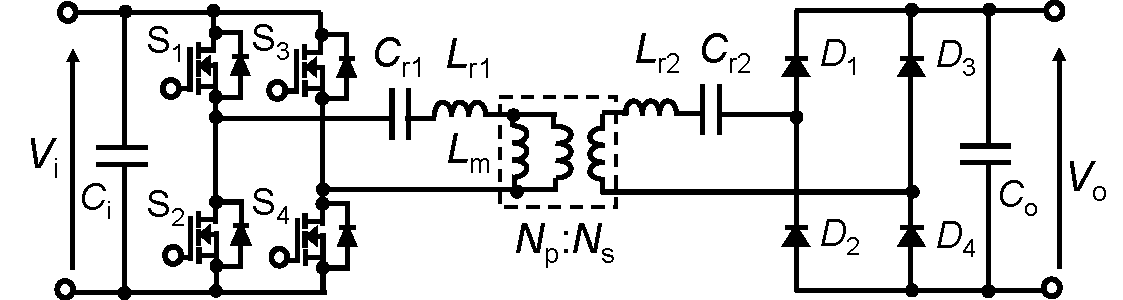
\includegraphics[width = \columnwidth]{figures_chapter2/setup.pdf}
    \caption{Circuit diagram used for simulation.} \label{fig:setup}
\end{figure}

Figure \ref{fig:100kWSim} shows the circuit simulation results at 100 kW for (a) 100\% load, (b) 50\% load, and (c) 20\% load. ZVS is achieved using the circuit parameters.

\begin{figure}[h!]
    \centering
    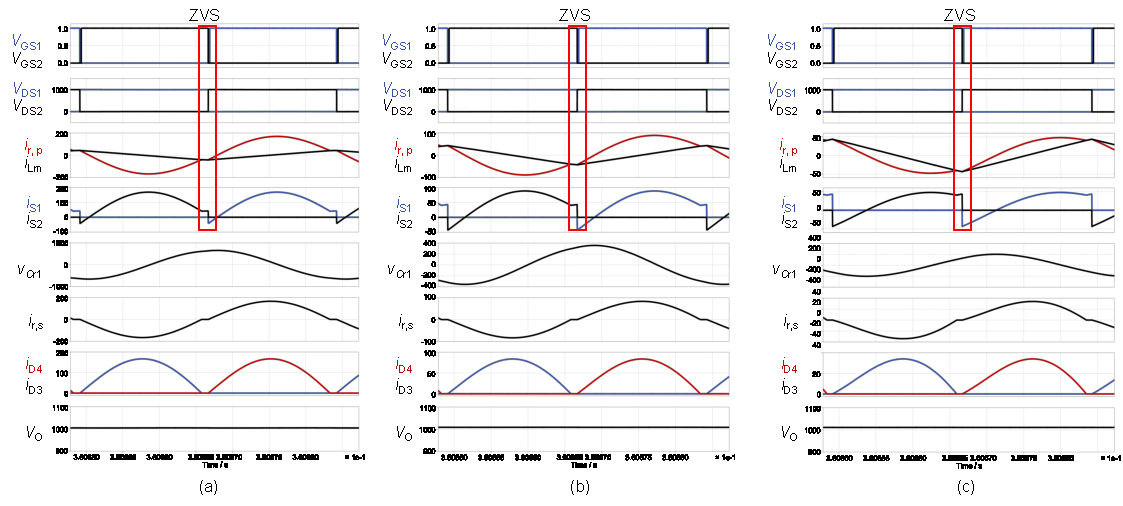
\includegraphics[width = \columnwidth]{figures_chapter2/100 kW compilation .pdf}
    \caption{100 kW circuit simulation results: (a) at 100\% load, (b) at 50 \% load, and (c) at 20\% load.} \label{fig:100kWSim}
\end{figure}

\pagebreak
Figure \ref{fig:1kWSim} shows the circuit simulation results at 1 kW for (a) 100\% load, (b) 50\% load, and (c) 20\% load. ZVS is achieved using the same resonant tank with the 100 kW circuit.

\begin{figure}[h!]
    \centering
    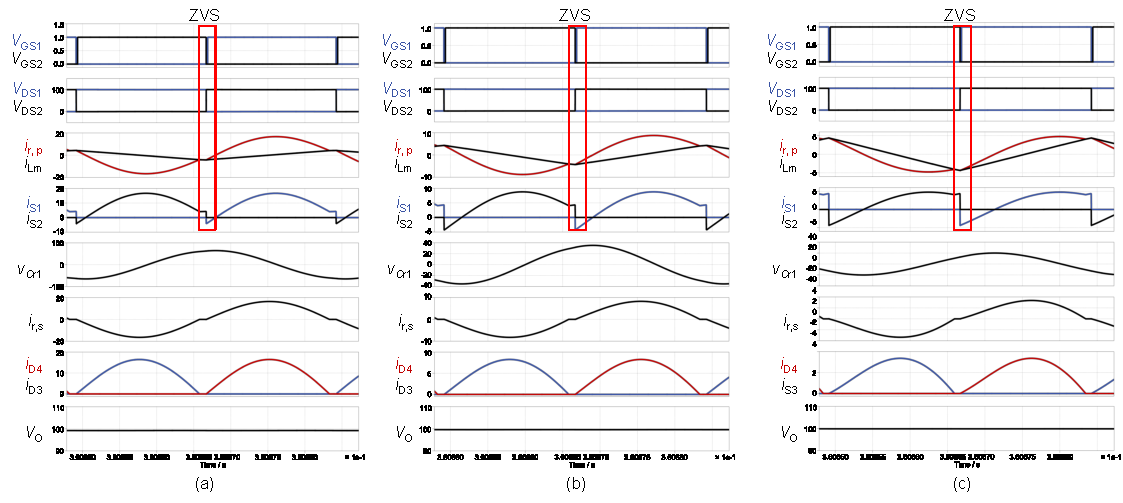
\includegraphics[width = \columnwidth]{figures_chapter2/1 kW compilation.pdf}
    \caption{1 kW circuit simulation results: (a) at 100\% load, (b) at 50 \% load, and (c) at 20\% load.} \label{fig:1kWSim}
\end{figure}

\pagebreak
For reference, the electrical circuit parameters used in the study are detailed in Table \ref{tab:power_electrical}, including the scalability analysis.

\begin{table}[h!]
\centering
\caption{Electrical Specifications for the Study}
\label{tab:power_electrical}
\begin{threeparttable}
\begin{tabular}{llccc}
\hline
\hline
\textbf{Parameter} & \textbf{Symbol} & \textbf{1 kW} & \textbf{10 kW} & \textbf{100 kW} \\
\hline
Input Voltage & $V_{\mathrm{in}}$ & 100 V & $316\text{ V } (\times\sqrt{10})$ & $1000\text{ V } (\times 10)$ \\
Output Voltage & $V_{\mathrm{o}}$ & 100 V & $316\text{ V } (\times\sqrt{10})$ & $1000\text{ V } (\times 10)$ \\
Output Current & $I_{\mathrm{o}}$ & 10 A & $31.6\text{ A } (\times\sqrt{10})$ & $100\text{ A } (\times 10)$ \\
Output Power & $P_{\mathrm{o}}$ & 1 kW & $10\text{ kW } (\times 10)$ & $100\text{ kW } (\times 100)$ \\
Switching Frequency\tnote{a}& $f_{\mathrm{sw}}$ & 15 -- 30 kHz & 15 -- 30 kHz & 15 -- 30 kHz \\
Resonant Frequency & $f_{\mathrm{r}}$ & 30.0 kHz & 30.0 kHz & 30.0 kHz \\
Dead Time & $t_{\mathrm{d}}$ & 360 ns & 360 ns & 360 ns \\
Resonant Capacitance & $C_{\mathrm{r1}}, C_{\mathrm{r2}}$ & $1.4~\upmu\text{F}$ & $1.4~\upmu\text{F}$ & $1.4~\upmu\text{F}$ \\
Resonant Inductance & $L_{\mathrm{r1}}, L_{\mathrm{r2}}$ & $20.1~\upmu\text{H}$ & $20.1~\upmu\text{H}$ & $20.1~\upmu\text{H}$ \\
Magnetizing Inductance & $L_{\mathrm{m}}$ & $200~\upmu\text{H}$ & $200~\upmu\text{H}$ & $200~\upmu\text{H}$ \\
\hline
\hline
\end{tabular}

\begin{tablenotes}
\small
\item[a] An $f_\mathrm{sw}$ of 28.5 kHz is chosen for this study.
\end{tablenotes}
\end{threeparttable}
\end{table}